\section{Benchmark Design}
\label{sec:method}

\textbf{Scoring methodology.}
Let a Robo2VLM test item be $(x_i,q_i,C_i,y_i)$, where $x_i$ is an RGB robot image, $q_i$ is a natural-language question, $C_i=\{c_{iA},\ldots,c_{iE}\}$ is a multiple-choice set, and $y_i$ is the correct option letter. We curate each item into a label
\begin{equation}
    \ell_i \in \{\mathrm{spatial},\mathrm{affordance},\mathrm{discarded}\},
\end{equation}
then assign deterministic subcategories from question text. Spatial questions are grouped into depth/distance ordering, directional orientation, and cross-view correspondence questions. Affordance questions are grouped into object blockage/reachability and grasp stability questions. Goal-state matching and task-completion questions are discarded because they test task-state recognition rather than spatial reasoning or affordance understanding.

For a model $M$, prompt mode $p$, and optional image transform $a$, for example adding depth information, the evaluator forms the prompt
\begin{equation}
    z_i = p(q_i,C_i), \qquad r_i = M(a(x_i),z_i),
\end{equation}
extracts the last standalone letter in $\{A,B,C,D,E\}$ from $r_i$, and computes
\begin{equation}
    \mathrm{Acc}(M,p,S) =
    \frac{1}{|S|}\sum_{i \in S}\mathbf{1}[\hat{y}_i=y_i].
\end{equation}
The two prompt modes are zero-shot (ZS), which requests only the option letter, and chain-of-thought (CoT), which asks for step-by-step reasoning followed by the final letter. Since CoT responses may contain several option letters in the reasoning text, the final standalone letter controls scoring.

\textbf{Curation and sampling.}
The curated Robo2VLM-1 test split contains 6,676 questions: 2,084 spatial, 842 affordance, and 3,750 discarded out-of-scope questions. Deterministic subcategory counts are shown in \cref{tab:curation}, and representative data samples are shown in \cref{fig:data-samples}.

\begin{table}[t]
  \centering
  \small
  \setlength{\tabcolsep}{4pt}
  \begin{tabular}{@{}llr@{}}
    \toprule
    Label & Subcategory & Count \\
    \midrule
    Spatial & depth/distance ordering & 1,283 \\
    Spatial & directional orientation & 798 \\
    Spatial & other spatial & 3 \\
    Affordance & object blockage/reachability & 543 \\
    Affordance & grasp stability & 299 \\
    Discarded & out of scope & 3,750 \\
    \bottomrule
  \end{tabular}
  \caption{Curated Robo2VLM-1 test split used to construct the evaluation subsets.}
  \label{tab:curation}
\end{table}

\begin{figure*}[t]
  \centering
  \begin{subfigure}[t]{0.48\linewidth}
    \centering
    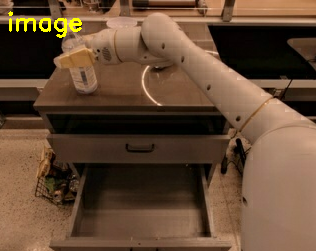
\includegraphics[width=\linewidth]{figures/sample_source_0000_bottle.png}
    \caption{Object blockage/reachability, source 0.}
  \end{subfigure}
  \hfill
  \begin{subfigure}[t]{0.48\linewidth}
    \centering
    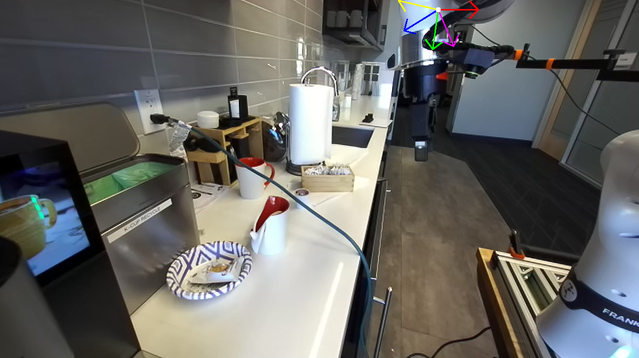
\includegraphics[width=\linewidth]{figures/sample_source_0368_directional_orientation.png}
    \caption{Directional orientation, source 368.}
  \end{subfigure}
  \vspace{3pt}

  \begin{subfigure}[t]{0.48\linewidth}
    \centering
    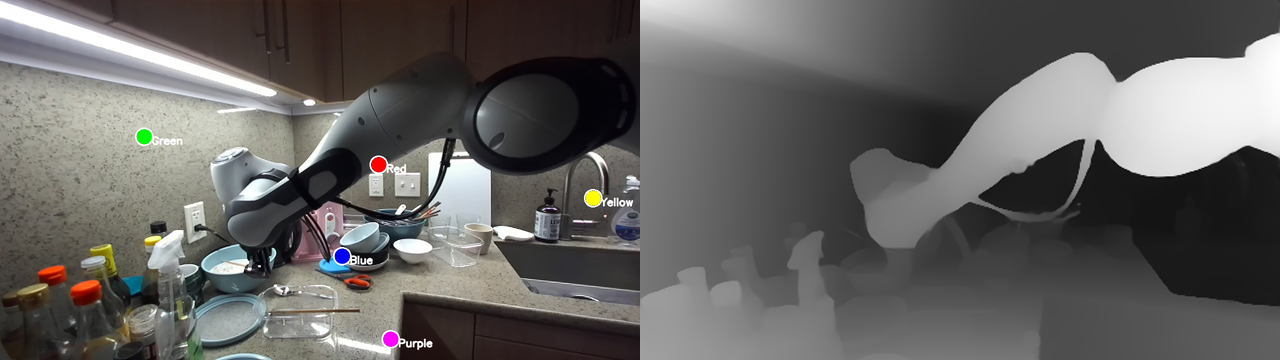
\includegraphics[width=\linewidth]{figures/sample_source_0407_depth_ordering.png}
    \caption{Depth/distance ordering, source 407.}
  \end{subfigure}
  \hfill
  \begin{subfigure}[t]{0.48\linewidth}
    \centering
    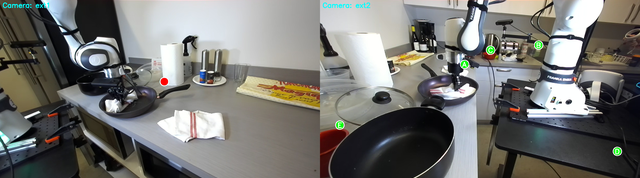
\includegraphics[width=\linewidth]{figures/sample_source_0408_cross_view.png}
    \caption{Cross-view correspondence, source 408.}
  \end{subfigure}
  \caption{Actual Robo2VLM examples used to ground the benchmark categories. The images show why aggregate VQA accuracy is insufficient: the benchmark mixes reachability judgments, end-effector directional orientation, depth ordering from overlaid points, and correspondence across camera views. The first panel also corresponds to the DeepSeek CoT failure in \cref{tab:evidence}, where the model treats the target bottle itself as an obstacle.}
  \label{fig:data-samples}
\end{figure*}

\textbf{Sanity probes.}
The scored runs are complemented by raw-generation probes over 20 spatial CoT examples per model. For each example, we ask the model to justify the correct answer on the original image, assess a deliberately wrong answer, assess the correct answer on a blank image, assess the correct answer on a shuffled mismatched image, and describe overlays without selecting an answer. A phrase-based heuristic labels each response as supporting, rejecting/insufficient, or unclear. These labels are for triage, not a substitute for manual grounding evaluation.

\textbf{Human performance evaluation.}
To complement the automated model evaluation, a human performance study was conducted on a subset of the benchmark. This analysis was motivated by the observation that the evaluated vision-language models exhibited only marginal performance differences across settings, prompting a closer inspection of the dataset itself. A manual review revealed that a subset of samples contains ambiguities, incomplete visual information, or inherently under-specified questions, which can make them challenging even for human annotators.

To quantify the impact of such issues, a random subset of 50 question–image pairs was selected from the curated dataset and presented to a group of human participants. The participants were asked to answer each question based solely on the provided image and task description, without access to external information or prior context.
